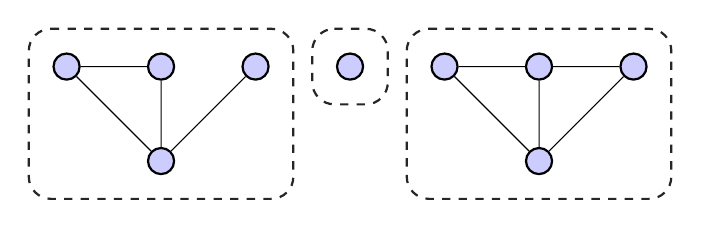
\begin{tikzpicture}
[scale=.6,auto=left,every node/.style={circle,fill=blue!20,draw=black,thick}]

  % Componente izquierda
  \node (n1) at (0,2) {};
  \node (n2) at (2,2) {};
  \node (n3) at (2,0) {};
  \node (n4) at (4,2) {};

  \foreach \from/\to in {n1/n2,n1/n3,n2/n3,n3/n4}
    \draw (\from) -- (\to);

  % Vértice aislado central
  \node (n5) at (6,2) {};

  % Componente derecha
  \node (n6) at (8,2) {};
  \node (n7) at (10,2) {};
  \node (n8) at (10,0) {};
  \node (n9) at (12,2) {};

  \foreach \from/\to in {n6/n7,n6/n8,n7/n8,n7/n9,n8/n9}
    \draw (\from) -- (\to);

  % --- Envolventes estilo mano alzada rectangulares ---
  \begin{scope}[
    dashed,
    black!85, % Color más oscuro
    thick,
    decorate,
    decoration={random steps, segment length=5mm, amplitude=1.2mm}
  ]
    % Envolvente izquierda (cuadrada/rectangular)
    \draw[rounded corners=8pt] 
      (-0.8,2.8) -- (4.8,2.8) -- (4.8,-0.8) -- (-0.8,-0.8) -- cycle;

    % Envolvente centro (alrededor de n5)
    \draw[rounded corners=8pt] 
      (5.2,2.8) -- (6.8,2.8) -- (6.8,1.2) -- (5.2,1.2) -- cycle;

    % Envolvente derecha (cuadrada/rectangular)
    \draw[rounded corners=8pt] 
      (7.2,2.8) -- (12.8,2.8) -- (12.8,-0.8) -- (7.2,-0.8) -- cycle;
  \end{scope}

\end{tikzpicture}
